\documentclass[11pt]{article} 
\usepackage{a4wide,url,graphicx}

\title{The \SD\ GEO Records --\\ A Public Repository of Geometry Theorem Proof
  Schemes}

\author{Hans-Gert Gr\"abe, Univ. Leipzig, Germany}

\date{November 26, 2002}

\newcommand{\GC}{\textit{Geo\-Code}} 
\newcommand{\GP}{\textit{Geo\-Prover}}
\newcommand{\SD}{\textit{Symbolic\-Data}} 
\newcommand{\gf}[1]{{\tt #1}\/}
\newcommand{\formel}[1]{\[\begin{array}{l}#1\end{array}\]}
\newcommand{\extendedgeocode}[2] {{\tt #1}\\[1pt]\hsp\parbox{11cm}{#2}\\[6pt]}
\renewcommand{\topfraction}{0.95} 
\newcommand{\hsp}{\hspace*{1cm}}

\begin{document}

\maketitle

\section{Introduction}

Geometry is not only a part of mathematics with ancient roots but also a vivid
area of modern research. Especially the field of geometry called by some
negligence ``elementary'' continues to attract the attention also of the great
community of leisure mathematicians.  This is probably due to the small set of
prerequisites necessary to formulate the problems posed in this area and the
erudition and non formal approaches ubiquitously needed to solve them.
Examples from this area are also an indispensable component of high school
mathematical competitions of different levels upto the International
Mathematics Olympiad (IMO) \cite{IMO}.  \medskip

The great range of ideas being involved with elementary geometry theorem
proving inspired mathematicians to search for a common framework that allows
to discover such geometric statements or, at least, to prove them in a more
unified way. These attempts may be traced back until ancient times, e.g., to
Euclid and his axiomatic approach to geometry.

A special common framework for geometry theorem proving was known at least
since Descartes and his coordinate method: Translate geometric configurations
into algebraic relations between coordinates and try to solve the algebraic
counterpart of the geometric problem by algebraic methods. It was this
framework that inspired the young Gauss for his famous solution to construct a
regular 17-gon by ruler and compass.

With the increasing capabilities of modern computer equipment to do term
rewriting and symbolic algebraic manipulations this approach obtained new
power. The surprising observation that tedious but mostly straightforward
algebraic manipulations allow to derive (mathematically strong!) proofs for
many theorems in geometry with even ingenious ``true geometric'' proofs led
many researchers to focus anew on questions of automated deduction of
geometric statements.

The attempts to algorithmize this part of mathematics found their first
culmination in the 80's in the work of W.-T.~Wu on ``the Chinese Prover'',
see, e.g., \cite{Wu_84a, Wu_84b} and the surveys in \cite{Books/Wu_94a} or
\cite{Wu_99a}. In the following these ideas were largely extended by different
people, among them the ``Chinese provers'' in Wu's school at MMRC.  Let's
mention only the remarkable book \cite{Books/Chou_88a} of S.-C.~Chou who
proved 512 geometry theorems with this mechanization method.

There are two conclusions to be drawn from Chou's book. First, the
applicability of algebraic methods to geometry theorem proving is really
convincing. A surprisingly great number of examples fall into the class of
{\em constructive} problems ({\em explicitely constructive} in
\cite{Books/Wu_01a}), where the geometric configuration can be constructed
step by step in such a way that new coordinates depend rationally on (free
parameters and) coordinates of already constructed objects and the geometric
conclusion translates into a rational expression in these coordinates that
should vanish. In this situation the solution of the algebraic problem reduces
to a zero simplification problem of a rational expression in several
(algebraically independent) variables.  This problem is well understood and
admits an efficient solution that is implemented in the core of all major (and
minor) Computer Algebra Systems (CAS).  Nevertheless real such simplifications
may be very time and memory consuming, so that in some cases a
non-constructive algebraic translation has to be preferred.

The coordinate method yields mathematically strong proofs for geometric
statements with a serious drawback: Due to the algebraic nature of the
intermediate steps these proofs cannot be retranslated to geometric reasoning
but for a small number of cases.  Often the algebraic statements ``fit
together'' but the underlying geometry remains ``invisible''.  More geometric
approaches are discussed, e.g., in \cite{Books/Chou_94a}. They still use
polynomial computations, but take geometric invariants like areas and
Pythagoras differences instead of coordinates of points as the basic
quantities. Thus the geometric meaning for each step of the proof is clear.

Second, the proofs are not ``automated'' but ``mechanized'' in the following
sense: A partly informal human readable geometric statement requires a
translation into a strong computer readable syntax.  In Chou's book
\cite{Books/Chou_88a} these {\em proof schemes} or {\em coordinatizations},
i.e., descriptions of geometric configurations of points, lines, and circles
in a syntactically strong way, are composed by the author in a LISP like
language and afterwards translated to their algebraic counterparts by the
computer.  For some theorems the given coordinatization is quite tricky, since
the algebraic translation of the ad hoc solution is too hard to be handled by
the computer.  Even though speaking about ``automatic geometry
problem-solving'' (\cite{Wu_99a}), also Wu emphasizes (on p.~12 of that paper
and even in the title of \cite{Books/Wu_94a}) on ``mechanization methods''
rather than ``automated deduction'' in full accordance with modern concepts of
human-computer interaction. Such concepts consider computers not as automata
but as tools in a more complex human-computer environment that combines
precision and speed of computer equipment with human creativity and (informal)
experience.
 
Mechanization of geometry theorem proving hence requires the creativity of
diligent ``proof writers'' to eliminate all informal elements from a geometric
statement and to fix the result in a (completely formalized) geometric proof
scheme.  These proof schemes are the starting point for further automated
translation to, e.g., algebraic statements.

For intercommunication purposes and to store proof schemes in a common
publicly available repository it is necessary to develop a {\em generic proof
  scheme language standard} that can be implemented with appropriate tools by
all interested parties.  In this paper we describe a first approach to such a
standard, the {\em {\GC}}. It is used to store proof schemes as GEO records in
a repository that is publicly available as part of the \SD\ Project
\cite{SymbolicData}.  At the moment the \SD\ GEO collection contains more than
250 such proof schemes, mainly from \cite{Books/Chou_88a}.  Special \SD\ tools
are designed to support the syntactical translation of {\GC} into proof scheme
languages of special geometry theorem provers that support this common
interface.  At the moment -- as a first reference application -- this
interface is implemented in the author's \GP\ packages \cite{GeoProver}, that
provide tools to run proof scheme translations based on the coordinate
method on one of the major CAS (Maple, Mathematica, MuPAD, Reduce).

The {\GC} standard evolved in a tight interplay between the collection of
proof schemes and their evaluation with different versions of the {\GP} on
different platforms. As a result of the discussions at the conference ADG-02
the standard was revised once more in the following directions:
\begin{enumerate}
\item The proof schemes collected so far used algebraic expressions to detect
  equality of angles, segments, triangle areas etc. To serve also more
  geometric approaches (e.g., the area method) these algebraic expressions
  were substituted by function calls with clear geometric meaning like {\tt
    Equal}, {\tt eqdist} etc. 
\item The {\GC} standard uses {\tt Point}, {\tt Line} and {\tt Circle} as
  geometric types.  Since most of the geometry theorem provers take points as
  basic primitives and consider lines and circles as derived objects, the
  constructors {\tt Line}$[a_1,a_2,a_3]$ and {\tt Circle}$[c_0,c_1,c_2,c_3]$
  were removed from the standard.
  
  Moreover, the definition of free points was singled out into a special
  attribute {\tt Points} of the GEO proof scheme record to separate them from
  true geometric construction steps.
\item The names of the {\GC} functions were adjusted once more. 
\end{enumerate}
Since the {\GC} description is fixed in the same \SD\ format as the GEO
records themselves such adjustments are well supported by the {\SD} action
concept and the Perl string manipulation facilities. This allows to write
compact Perl scripts to execute the required changes in the GEO proof scheme
records.  
\medskip

This paper starts with some background on geometry theorem proving (section
2). Then we describe the design of the GEO records, the syntax of the {\GC}
standard and the {\GP} packages as an implementation of that standard (section
3). In section~4 we discuss by means of examples how to compile new (generic)
proof schemes, to translate them into \GP\ notion, to run this code on
different CAS and to experiment with the resulting algebraic problems.

For real usability of the {\GC} concept one has to estimate the efforts
required to implement this standard for other provers.  Even though there is
not yet practical experience with already existing geometry theorem provers
the semantic similarity of ``foreign'' special geometric proof schemes
suggests that such an interface should easily to be implemented.  The problem
is discussed in more detail in section~5 on the special geometric language
used in \cite{Wang_97a} and, in a slightly revised form, also in D.Wang's
GEOTHER project \cite{Geother}, see also \cite{Wang_96b}.
\medskip

A main problem to translate GEO records into geometric proof schemes for
special geometry theorem provers is posed by different programming paradigms
followed by the underlying geometry theorem provers. The {\GC} standard
supports a functional programming style and the GEO record attribute values
heavily use nested function calls. Several provers and dynamical geometry
softwares (DGS) do not support nested function calls since they create and
address geometric objects through identifiers.

We studied that problem within the task to translate our (constructive) proof
schemes also to {\em construction schemes} that can be interpreted by DGS to
draw a picture of the given geometric configuration or to generate a human
readable {\em construction plan}. Such facilities are part of integrated
geometry theorem provers as, e.g., D.~Wang's GEOTHER prover \cite{Geother,
  Wang_96b} or the {\em Geometry Expert}, \cite{gex}. We developed a first
(Perl based) prototype interface of constructive GEO proof schemes to the
{GEONE$_X$T} system \cite{Geonext} that really denests nested function calls.

\section{Geometry Theorem Proving and the Coordinate Method}

As already described in the introduction the main approach to mechanized
geometry theorem proving considered so far depends on Descartes-Wu's
coordinate method, translates geometric statements into their algebraic
counterparts, i.e., statements about systems of polynomial or rational
functions, and tries to solve these algebraic problems by algebraic methods.

\subsection{Geometry Theorems of Constructive Type}

Usually geometric constructions can be compiled from a small number of
elementary constructions, e.g., drawing a line through given points,
constructing intersection points, circles with given parameters etc.  In the
same way also the coordinate representation of geometric statements can be
produced cascading only a small number of elementary functions and data types.
Hence interpreting the function calls in a geometric proof scheme in such an
algebraic manner yields its algebraic translation as the starting point for
the application of algebraic methods.

Note that the same proof scheme can be interpreted in a completely different
way, e.g., by a drawing tool or geometry theorem prover based on a different
method. This aspect will be discussed below.  In this section we identify
proof schemes and their algebraic translations. 

We use points, lines and circles as basic objects with symbolic or numerical
coordinates:
\begin{quote}
\begin{tabular}{ll}
$(x,y)$ & the point $(x,y)$,\\
$(g_1,g_2,g_3)$ & the line $\{(x,y)\,:\, g_1\,x+g_2\,y+g_3=0\}$, and\\
$(c_1,c_2,c_3,c_4)$ & the circle $\{(x,y) \,:\,
c_1\,(x^2+y^2)+c_2\,x+c_3\,y+c_4=0 \}$.
\end{tabular}
\end{quote}
Let $\gf{midpoint}(X,Y)$ be the midpoint of the segment ${XY}$,
$\gf{pp\_line}(X,Y)$ the line through $X$ and $Y$ and
$\gf{is\_concurrent}(a,b,c)$ a polynomial condition (in fact, a determinantal
expression) that vanishes iff the lines $a,b,c$ pass through a common point.
The return values of all these functions are (sequences of) rational
expressions in the coordinates of the formal input parameters.  \medskip

With these functions at hand, e.g., the centroid intersection theorem can be
proved in the following way: Choose generic points
\[A:=\gf{Point}(u_1,u_2);\quad B:=\gf{Point}(u_3,u_4);\quad
C:=\gf{Point}(u_5,u_6);
\] 
compute coordinates for 
\[A_1:=\gf{midpoint}(B,C);\quad B_1:=\gf{midpoint}(A,C);\quad
C_1:=\gf{midpoint}(A,B);
\]
and evaluate the statement
\begin{equation}\label{centroid}
\gf{is\_concurrent}(\gf{pp\_line}(A,A_1), \gf{pp\_line}(B,B_1),
\gf{pp\_line}(C,C_1))
\end{equation}
To prove this theorem (and other theorems of this type) means to compose a
nested rational expression like (\ref{centroid}) and to check if it simplifies
to zero. If it does, it will simplify to zero also for (almost) all {\em
  special} geometric configurations obtained from the {\em generic}
configuration plugging in special numerical values for $u_1,\ldots,u_6$.
\medskip

In general, we say that a geometric configuration is of {\em constructive
  type}, if its generic configuration can be constructed step by step in such
a way, that the coordinates of each successive geometric object can be
expressed as rational functions in the coordinates of already constructed
objects and algebraically independent variables, and the conclusion can be
expressed as vanishing of a rational function in these coordinates.

Such a theorem is generically true if and only if its configuration is not
contradictory and the conclusion expression simplifies to zero.

Note that due to Euclidean symmetry even for generic configurations some of
the coordinates can be chosen in a special way.

\subsection{Geometry Theorems of Equational Type}

Surprisingly many geometry theorems can be translated into statements of
constructive type.  Problems cause geometric objects derived from non-linear
geo\-metric conditions (angles, circles) if they are not uniquely defined or
their coordinates cannot be rationally expressed in the given indeterminates.
Geometric configurations with such objects require other proof techniques.

For example, given generic points $A=\gf{Point}(a_1,a_2),
B=\gf{Point}(b_1,b_2), C=\gf{Point}(c_1,c_2),$ a point $P=\gf{Point}(x_1,x_2)$
is on the bisector of the angle $\angle\,ABC$ iff $\angle\,ABP=\angle\,PBC$,
or, in \GP\ notation, iff
\formel{\gf{l2\_angle}(\gf{pp\_line}(A,B),\gf{pp\_line}(P,B)) =%\\[8pt]\hsp\hsp
  \gf{l2\_angle}(\gf{pp\_line}(P,B),\gf{pp\_line}(C,B)) } In this formula
$\gf{l2\_angle}(g,h)$ denotes the tangens of the angle between the lines
$g=(g_1,g_2,g_3)$ and $h=(h_1,h_2,h_3)$ that can be computed as
$$\frac{g_2\,h_1-g_1\,h_2}{g_1\,h_1+g_2\,h_2}.$$

Clearing denominators this condition on $P$ translates into a polynomial of
(total) degree 4 in the generic coordinates and quadratic in the coordinates
of $P$.  It describes the condition {\tt on\_bisector(P,A,B,C)} for $P$ to be
on either the inner or the outer bisector of $\angle\,ABC$.  Note that in
unordered geometry there is no way to distinguish between the inner and outer
bisectors.

To prove the bisector intersection theorem lets ``compute'' the coordinates of
the intersection points $P$ of the bisectors through $A$ and $B$ and show that
they belong to (one of) the bisectors through $C$.  Due to Euclidean symmetry
we can choose special coordinates for $A$ and $B$ to simplify calculations.
\begin{quote}
\begin{verbatim}
A:=Point(0,0);  B:=Point(1,0);  C:=Point(u1,u2); P:=Point(x1,x2);

polys:={on_bisector(P,A,B,C), on_bisector(P,C,A,B)};
\end{verbatim}
\end{quote}\vspace{-8pt}
\formel{\big\{ -2\,{x_2}+2\,{u_1}\,{x_2}+2\,{x_2}\,{x_1}
  -2\,{x_2}\,{u_1}\,{x_1} -{u_2}\,{{x_2}}^{2}+{u_2}-2\,
  {u_2}\,{x_1}+{u_2}\,{{x_1}}^{2},\\[4pt]\hsp 2\,{x_2}\,{u_1}\,{x_1}
  -{u_2}\,{{x_1}}^{2}+{u_2}\,{{x_2}}^{2}\big\}} 
{\tt polys} is a system of two polynomial equations of degree 2 in $(x_1,x_2)$
with coefficients in ${\bf Q}(u_1,u_2)$. It has 4 solutions that correspond to
the 4 intersection points of the bisector pairs through $A$ and $B$. They can
be computed, e.g., with Maple:
\begin{quote}
\begin{verbatim}
solve(polys,{x1,x2});
\end{verbatim}
\end{quote}
\[\left\{ {x_2}=\%1, {x_1}=1/2\,{\frac {{ u_2}-2\,\%1
      +2\,{u_1}\,\%1 }{{u_2}-\%1}}\right\}\] \formel{\%1 = {\it RootOf} \left(
    4\,{u_2}\,{{\it \_Z}}^{4}+ \left( -8\,{{u_1}}^{2}-8\,{{u_2}}^{2}+8\,{u_1}
    \right) {{ \it \_Z}}^{3} \right. \\\hsp\left.  + \left( -4\,{u_1}\,{u_2}
      +4\,{{u_1}}^{2}{u_2} -4\,{u_2} +4\,{{u_2}}^{3} \right) {{\it \_Z}}^{2}
    +4\,{{u_2}}^{2}{\it \_Z}-{{u_2}}^{3} \right)} The solution involves
algebraic {\it RootOf\/}-expressions that require a powerful algebraic engine
to cope with.

Another approach uses direct reformulation of the geometry theorem as a
vanishing problem of the polynomial conclusion on the zero set of the system
of polynomials that describe the given geometric configuration.

For our example, consider the conclusion polynomial
\begin{quote}
\begin{verbatim}
con:=on_bisector(P,B,C,A);
\end{verbatim}
  $2\,{{u_1}}^{2}{x_2}\,{x_1}+2\,{u_2}\,{{x_2}}^{2}{u_1}
  -2\,{u_2}\,{{x_1}}^{2}{u_1} -{u_2}\,{{x_2}}^{2} +{u_2}\,{{x_1}}^{2}
  +2\,{u_2}\,{x_1}\,{{u_1}}^{2} -2\,{{ u_2}}^{2}{x_1}\,{x_2}
  -2\,{x_2}\,{u_1}\,{x_1} -{{ u_1}}^{2}{u_2} +2\,{{u_2}}^{2}{x_2}
  -{{u_2}}^{3}+2\,{ x_2}\,{{u_1}}^{2} -2\,{{u_1}}^{3}{x_2} +2\,{{u_2}}^{3}{
    x_1} -2\,{u_1}\,{x_2}\,{{u_2}}^{2}$
\end{quote}
and check if it vanishes on the variety of zeroes of {\tt polys} regarded as
zero dimensional polynomial system in ${\bf Q}(u_1,u_2)[x_1,x_2].$ This
follows if the normal form of {\tt con} with respect to a Gr\"obner basis of
{\tt polys} vanishes.  Hence the following Maple computation verifies the
theorem:
\begin{quote}
\begin{verbatim}
with(Groebner):
TO:=plex(x1,x2): gb:=gbasis(polys,TO):
normalf(con,gb,TO);
\end{verbatim}
  \centerline{$0$}
\end{quote}
In general, this kind of algebraization of geometry theorems by the coordinate
method yields a polynomial ring $S=k[{\bf v}]$ with variables ${\bf v} =(v_1,
\ldots, v_n)$, a polynomial system $F\subset S$ that describes algebraic
dependency relations in the given geometric configuration, a subdivision ${\bf
  v} = {\bf x} \cup {\bf u}$ of the variables into dependent and independent
ones, and the conclusion polynomial $g({\bf x}, {\bf u}) \in S$.

A set of variables ${\bf u}$ is {\em independent} wrt.\ an ideal $I=I(F)$ iff
$k[{\bf u}]\cap I=(0)$, i.e., if {\bf u} is algebraically independent on the
variety $Z(F)$ of zeroes of $F$.  In most practical applications such a
subdivision is obvious.  A strong verification can be derived from a Gr\"obner
basis of $F$ wrt.\ an appropriate term order.

$Z(F)$ may be decomposed into irreducible components that correspond to prime
components $P_\alpha$ of the ideal $I = I(F)$ generated by $F$ over the ring
$S = k[{\bf x}, {\bf u}]$.  Since $P_\alpha\supseteq I$ the variables ${\bf
  u}$ may become dependent wrt.\ $P_\alpha$.  Prime components where ${\bf u}$
remains independent are called {\em generic}, the other components are called
{\em special}.  By definition, every special component contains a non zero
polynomial in the independent variables ${\bf u}$.  Multiplying them all
together yields a non degeneracy condition $h = h({\bf u}) \in k[{\bf u}]$ on
the independent variables such that a zero ${\bf c} \in Z(F)$ with $h({\bf
  c})\neq 0$ necessarily belongs to one of the generic components.  Hence they
are the ``essential'' components and we say that {\em the geometry theorem is
  generically true}, when the conclusion polynomial $g$ vanishes on all these
generic components.

If we compute in the ring $S_0 = k({\bf u})[{\bf x}]$ as we did in the above
example, i.e., consider the independent variables as parameters, exactly the
generic components of $I$ remain visible.  Hence if the normal form of $g$
wrt.\ a Gr\"obner basis $G$ of $F$ computed in $S_0$ vanishes the geometry
theorem is generically true.  More subtle examples can be analyzed with the
Gr\"obner factorizer or more advanced techniques.

There are other algebraic techniques to analyze such polynomial systems, e.g.,
based on pseudo division and triangular sets. See \cite{Kapur_97a} or the
monograph \cite{Books/Wang_01a} for a more complete survey.

\subsection{Mechanized Geometry Theorem Proving}

To really run mechanized geometry theorem proofs as described in the previous
subsection requires a target CAS and several ingredients:
\begin{itemize}\itemsep0pt
\item[(1)] We need a ``proof writer'' that writes (realistic) proof schemes
  for given informal statements of geometry theorems.
\item[(2)] We need tools to translate geometric statements into their
  algebraic counterparts as input for the target CAS.
\item[(3)] The CAS should be capable of the required algebraic manipulations.
\item[(4)] The CAS should provide tools to analyze the algebraic situation
  (e.g., to solve systems of equations, to compute Gr\"obner bases and normal
  forms etc.)
\end{itemize}

For Descartes-Wu's approach, topic (3) requires only facilities to compute
with rational expressions and is usually not the bottleneck for geometry
theorem proving.  For some proofs topic (4) may be really challenging since it
exploits the full compute power of the algebraic engine of the target CAS.
On the other hand different proof schemes for the same problem can yield
algebraic formulations of very different run time also within the same CAS.

In most cases topic (1) is straightforward, in particular if the informal
geometric statement is already highly constructive.  But in some applications
the ``proof writers'' had to develop really ingenious and non trivial ideas to
write reliable proofs that can be run automatically.  For example, Wu proposed
in \cite{Books/Wu_94a} the following constructive proof for the bisector
intersection theorem:
\begin{itemize}\itemsep0pt
\item Start with the vertices $A,B$ and the (future) intersection point $P$ of
  the bisectors through $A$ and $B$.
\item Draw the lines $c$ through $AB$, $d$ through $AP$ and $e$ through $BP$.
\item Draw lines $u,v$ derived from $c$ by reflection wrt.\ to the axes $d,
  e$.
  
  These lines will meet in a point $C$ such that $d$ and $e$ are the bisectors
  of $ABC$ through $A$ and $B$.
\item Prove that $P$ is also on the third bisector.
\end{itemize}
Geometry theorem prover usually provide tools for steps (2--4) to run proof
schemes written in a prover specific language automatically.  With a general
purpose CAS at hand it is enough to have tools for (2). Such translation tools
for Maple, MuPAD, Mathematica, and Reduce are provided by the author's {\GP}
packages, \cite{GeoProver}, see below.

The main drawback of all these systems is the restricted interoperability of
proof schemes.  To fix a proof scheme for automated processing by different
provers requires a generic language that can be mapped to all target systems.
Below we report about our experience with the {\GC} language that was invented
to store generic proof schemes in the {\SD} GEO record collection.  

Here is the notion of Wu's constructive proof scheme of the bisector
intersection theorem in {\GC} notation:
\begin{verbatim}
<Points> 
   $A:=Point[0,0]; $B:=Point[1,0]; $P:=Point[u1,u2]; 
</Points>
<coordinates>
   $l1:=pp_line[$A,$B];
   $l2:=sym_line[$l1,pp_line[$A,$P]];
   $l3:=sym_line[$l1,pp_line[$B,$P]];
</coordinates>
<conclusion> 
   $result:=on_bisector[$P,$A,$B,intersection_point[$l2,$l3]]; 
</conclusion>
\end{verbatim}
S.-C. Chou is probably one of the most diligent ``proof writers'' who
collected in \cite{Books/Chou_88a} more than 500 examples of geometric
statements and appropriate algebraic translations.

During our work on the \SD\ GEO collection we stored (and partly modified and
adapted) about 200 of them. We collected also solutions of geometry problems
from other sources, e.g., the IMO contests, see \cite{IMO}. Much of this work
was done by my ``proof writers'', the students Malte Witte and Ben Friedrich,
who compiled first electronic versions for many of these examples.

\section{{\GC} and GEO Records}

\subsection{The \SD\ Project}

The \SD\ project was set up to create and manage a publicly available
repository of digital test and benchmark data from different areas of symbolic
computation and to develop tools and concepts to manage such data both in the
repository and at a local site.  In a first stage we concentrated on the
development of practical concepts for a convenient data exchange format, the
collection of existing benchmark data from two main areas, polynomial system
solving and geometry theorem proving, and the development of appropriate tools
to process this data.  A tight interplay between conceptual work, data
collection, and tools (re)engineering allowed continuously to evaluate the
usefulness of each of the components.

For easy reuse we concentrated on free software tools and concepts.  The data
is stored in a XML like ASCII format that can be edited with your favorite
text editor.  The tools are completely written in Perl using Perl 5 modular
technology.

Some of our ad hoc concepts of data representation changed several times and
(although meanwhile being quite elaborated) surely will partly change in the
future (e.g., lists and hashes will probably be stored in a more XML compliant
form). Having data available in electronic form (so far) it was very easy to
translate it into the revised formats. Hence the most complicated part of the
project is the collection of benchmark data and its translation from the
foreign to the current format of the repository.  Note that our concept of
data representation is very flexible. The data format can be specified by the
user in an easy manner and very broad range. I refer to \cite{Bachmann_00a,
  karlsruhe-02, rwca-02} and the \SD\ documentation for more details.

The project is organized as a free software project. The CVS repository is
equally open to people joining the \SD\ project Group. Tools and data are
freely available also as tar-files from our Web site under the terms of the
GNU Public License.  
\medskip

The \SD\ project is part of the benchmark activities of the German
``Fachgruppe Computeralgebra'' who also sponsored the web site
\cite{SymbolicData} as a host for presentation and download of the tools and
data developed and collected so far.  We kindly acknowledge support also from
UMS MEDICIS of CNR/\'Ecole Polytechnique (France) who provides us with the
needed hard- and software to run this web site.  \medskip

\subsection{\SD\ Files and \SD\ Records}

Records in the \SD\ data base are stored as ASCII files ({\bf sd-files}) in a
(flat) XML like syntax. A typical example of such a record, the record
\verb|Parallelogram_2| in the GEO table, is given on page \pageref{table:1}.
It contains information and a mechanized proof scheme for the following
geometry theorem:
\begin{quote}\it
  The intersection point of the diagonals of a parallelogram is the midpoint
  of each of the diagonals.
\end{quote}

\begin{table}[p]\label{table:1}{
\begin{verbatim}
#######################################################
# Record 'GEO/Parallelogram_2'

<Id>        GEO/Parallelogram_2            </Id>
<Type>      GEO                            </Type>
<Key>       Parallelogram_2                </Key>
<prooftype> constructive                   </prooftype>
<parameters> [u1, u2, u3]                  </parameters>
<Points> 
$A:=Point[0,0]; $B:=Point[u1,0]; $D:=Point[u2,u3]; 
</Points>
<coordinates> 
$C:=par_point[$D,$A,$B];
$P:=intersection_point[pp_line[$A,$C],pp_line[$B,$D]];
</coordinates>
<conclusion> $result:=eqdist[$A,$P,$C,$P]; </conclusion>
<CRef>      
PROBLEMS/Geometry/Parallelogram => problem description 
</CRef>
<Version> ... </Version>
<ChangeLog>
Sep 7 2002 graebe: Translated to GeoCode 1.3
Sep 6 2002 graebe: new tag 'Points' created
Sep 2 2002 graebe: $C=par_point[..]
Feb 10 2002 graebe: translated to GeoProver 1.2 syntax
</ChangeLog>
<PERSON>    graebe                         </PERSON>
<Date>      Nov 1 1999                     </Date>
  
# End of record 'GEO/Parallelogram_2'
#######################################################
\end{verbatim}}
\centerline{The GEO record `Parallelogram\_2'}
\end{table}

Some of the attributes of that record ({\tt Type}, {\tt Key}, {\tt CRef},
\ldots) serve for identification or store relational information. The other
fields store the different parts of the proof scheme in {\GC} syntax.

Note that the description of the internal structure of these attributes is
given in the same format in a {\tt META/GEO} table.  Hence new attributes can
be added and existing attributes can be modified in an easy manner.

The sd-files are tight to Perl hashes ({\bf sd-records}) by the \SD\ tools in
a transparent way.  The \SD\ tools deliver such a hash object to the
application programmer for further Perl manipulation. An elaborated {\bf
  actions} concept reduces common programming overhead to a minimum.  Since
the detailed requirements of different user driven tasks are not known in
advance to the \SD\ developers it is difficult (and probably even not worth)
to design a more reliable interface.

\subsection{\SD\ Proof Schemes}

\SD\ GEO proof schemes are divided (roughly) into two types according to their
{\tt prooftype} attribute: constructive and equational.

The generic variables are provided as values of two attributes:
\begin{center}
\begin{tabular}{lp{12cm}}
\tt parameters & a list {\bf u} of independent parameters\\
\tt vars & a list {\bf x} of dependent variables (equational
proofs only) \\
\end{tabular}
\end{center}
For equational proofs the variable lists {\bf x} and {\bf u} are chosen in
such a way that {\bf u} is a maximal independent set of variables for the
given algebraic variety over $k[{\bf x}, {\bf u}]$ as defined above.

The basic attributes (with {\GC} values) are:
\begin{center}
\begin{tabular}{lp{12cm}}
\tt Points & the free points of the proof scheme\\
\tt coordinates & assignments that compose step by step the generic geometric
configuration of the proof scheme\\  
\tt conclusion & the conclusion of the proof scheme\\ 
\end{tabular}
\end{center}
This already completes the data required for a constructive proof scheme.  For
equational proof schemes the following additional attributes are defined:
\begin{center}
\begin{tabular}{lp{12cm}}
\tt polynomials & a list of {\GC} predicates that correspond to polynomial or
rational conditions describing algebraic dependency relations in the given
geometric configuration\\ 
\tt constraints & a list of {\GC} predicates that correspond to polynomial non
degeneracy conditions\\  
\tt solution & a way to solve the algebraic problem (given in extended {\GC}
syntax) 
\end{tabular}
\end{center}
The proof idea can be sketched within the {\tt ProofIdea} attribute as plain
text if not yet evident from the code. See \cite{rwca-02} for a detailed
description of the GEO record structure. Below we concentrate on the {\GC}
part.

\subsection{The {\GC} Syntax}

The design of the generic {\GC} language is mainly motivated by our aim to fix
geometry theorem proof schemes in such a way that they can easily be
translated to different target systems. A good but expensive idea would be to
define an appropriate (context free) programming language and to write cross
compilers or to invent a reliable (full) XML markup and to use style sheet
translations.  Since the syntaxes of the target languages are very similar we
decided to avoid these efforts and defined a generic language that can be
cross compiled using only regular patterns.  Due to its elaborated pattern
matching facilities Perl is best suited to realize this approach.  \medskip

We assume proof schemes to be composed by a sequence of assignments with
nested function calls as right hand sides that refer to previously defined
geometric objects and scalars as arguments. To be mapped to different target
systems the {\GC} language should meet the following requirements:
\begin{itemize}\itemsep0pt
\item[(1)] Variable, symbol and function names can be identified.
\item[(2)] The generic \GC\ can be mapped to the syntax of the target system
  without name clashes.
\end{itemize}

In this context the words `variable' and `symbol' are used in the following
sense: the former are `symbols with values' (e.g., names for points, lines,
circles), the latter `symbols without values' (i.e., names for parameters and
variables in the previous sense). It is a special peculiarity of symbolic
computations that these name spaces usually overlap.  For geometry theorem
proof schemes this overlap can be avoided. We use Perl like syntax (i.e., {\tt
  \char92\$[a-zA-z][a-zA-z0-9]*} in Perl regexp notation) for variable names
and small letter\,/\,digit combinations (i.e., {\tt [a-z][a-z0-9]*} in Perl
regexp notation -- we don't allow capital letters to avoid name clashes both
in Reduce and Mathematica) for symbol names.

Most CAS use parentheses both to group arithmetic expressions and argument
lists in function calls. Since this cannot be distinguished within a regular
language we use the Mathematica convention (i.e., brackets) for function call
notation\footnote{Note that most of the arithmetic expressions were replaced
  by new geometric predicates {\tt Equal}, {\tt eqdist}, {\tt Normal} etc.\ in
  the GEO records during preparation of version 1.3 (finished after the ADG-02
  conference) to emphasize the geometric nature of the proof schemes. }.

Equational GEO records usually contain also a {\tt solution} tag with a
description how the algebraic task can be solved. This description is fixed in
an extended \GC\ syntax. Interface packages for Maple, MuPAD, Mathematica, and
Reduce to map these generic commands to appropriate constructs are part of the
\SD\ distribution.  For details see \cite{rwca-02}.  \medskip

The names and signatures of all the {\GC} functions are stored in the \SD\ 
{\tt GeoCode} table and can be extracted, extended and modified in the same
way as other sd-records. Two such {\tt GeoCode} records are reproduced below.
The first one corresponds to an 'inline' function that requires a special
implementation, the second one to a 'macro' with a generic definition in {\GC}
syntax as value of the {\tt code} attribute that can be used to create an
implementation automatically. For a complete description of all functions see
the \SD\ {\tt GeoCode} documentation.

\begin{table}[p]\label{table:2}{
\begin{verbatim}
########################################################
# Record 'GeoCode/pp_line' 

<Id>        GeoCode/pp_line                </Id>
<Type>      GeoCode                        </Type>
<Key>       pp_line                        </Key>
<call>      pp_line[$A::Point,$B::Point]::Line </call>
<verbose>   line through A and B           </verbose>
<description> 
The line through <math>A</math> and <math>B</math>. 
</description>
... 

# End of record 'GeoCode/pp_line'
########################################################

########################################################
# Record 'GeoCode/altitude'

<Id>        GeoCode/altitude               </Id>
<Type>      GeoCode                        </Type>
<Key>       altitude                       </Key>
<call>      altitude[$A::Point,$B::Point,$C::Point]::Line </call>
<verbose>   altitude from A onto g(BC)     </verbose>
<code>      ortho_line[$A,pp_line[$B,$C]]  </code>
<description> 
The altitude from <math>A</math> onto <math>g(BC)</math>. 
</description>
...

# End of record 'GeoCode/altitude'
########################################################

\end{verbatim}}
\centerline{The {\tt GeoCode} records 'pp\_line' and `altidute'}
\end{table}

\subsection{The \GP\ Packages}

Really to run proof schemes written in {\GC} syntax with a geometry theorem
prover requires to translate the {\GC} to equivalent code in the special
language of the target prover. We propose the following approach: First, write
Perl tools to translate the generic proof scheme into a syntactic form that is
more appropriate for the target system (e.g., change square bracket, fix
variable and function names, etc.). This is well supported by the {\SD}
actions concept and sample implementations for such translators in the {\tt
  bin/GEO} directory of the {\SD} distribution.

Second, write an interface package in the language of the target prover that
maps the {\GC} functions to the prover specific functions.  The author's {\GP}
packages implement such interfaces for Maple, MuPAD, Mathematica, and Reduce.

For each of these CAS the \GP\ (formerly {\it Geometry\/}) provides a small
package for mechanized (plane) geometry manipulations with non degeneracy
tracing and a set of functions to handle generic and special geometric
configurations containing points, lines and circles.

For a flavor of the usage resp.\ a formal description of all functions see
the sample calculations in the previous section and the documentation
\cite{GeoProver}.  For some target systems there is also a plot extension that
allows to draw graphics from scenes, i.e., (of course special) geometric
configurations.

A first prototype of the {\GP} grew out from a course of lectures for students
of computer science on this topic held by the author at the Univ.\ of Leipzig
in fall 1996. It was updated and completed to version 1.1 of a Reduce package
after a similar lecture in spring 1998.  Later on in cooperation with Malte
Witte, at those times one of my students, the package was translated to the
other target systems.

Since version 1.2 there is a separate description of the \GC\ language that
was fixed in \SD\ format and added as the {\tt GeoCode} table to the \SD\ 
Project later on.  Now the complete {\GP} source code is generated from a
platform-specific 'inline' code part for the basic functions and generic {\GC}
{\tt code} values for advanced functions using special \SD\ tools.  This
facilitates a concise code management of the {\GP} source code if the {\GC}
standard changes during development.

\section{Some Examples}

To get a look and feel about the efforts required to compile new \GC\ proof
schemes, to translate them with \SD\ tools to \GP\ applications and to run
them on different target CAS let's consider some examples.

\subsubsection*{1. The ``cathedral example'', \cite[5.3]{Kapur_97a}} 

\parbox[b]{7cm}{\centering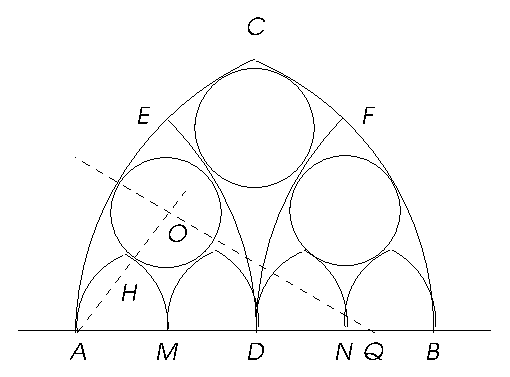
\includegraphics[width=6cm]{linz-02/gothic.eps}\\
Figure 1: The ``cathedral example''\vskip10pt}\hfill 
\parbox[b]{8cm}{\it $P, Q$ are centers of the arcs $CB, AC$, respectively;
  arcs $DE, DF$ are drawn with $R, S$ as centers, respectively, and $AQ$ as
  the radius. Further, $AQ=BP=\frac56 AB$.  The goal is to find the radius of
  the circle tangent to arcs $EA,ED,HM$ (with center $A$) and $KM$ (with
  center $D$) as a function of $AB$.\vskip40pt}

We take the problem formulation and notational conventions from
\cite{Kapur_97a} with $s=|\overline{AB}|=1$.  In that paper line $AB$ is taken
as $x$-axis with origin at $M$ (written as {\tt \$M} in \GC\ syntax) and the
following coordinates are assigned to points (using the \GC\ point
constructor):
\begin{verbatim}
$O:=Point[0,y3]; $A:=Point[-3/12,0]; $Q:=Point[7/12,0]; $M:=Point[0,0];
\end{verbatim}
Kapur's original proof scheme contains 6 algebraic conditions that arize from
the tangency conditions of two circle pairs.  A circle tangency condition
yields 3 polynomials: If $T_1=(x_1,y_1)$ is the point of tangency of the
circles around $A$ and $O$ these conditions are '$T_1$ on the circle around
$A$', '$T_1$ on the circle around $O$', and '$T_1, A, O$ are collinear'.

Here is that statement in the formal \GC\ syntax:
\begin{verbatim}
<vars>      [x1,y1,x2,y2,y3,r]                        </vars>
<Points>
   $O:=Point[0,y3]; $A:=Point[-1/4,0]; $Q:=Point[7/12,0]; $M:=Point[0,0]; 
   $T1:=Point[x1,y1]; $T2:=Point[x2,y2]; 
</Points>
<coordinates> 
   $c1:=pc_circle[$A,$M]; $c2:=pc_circle[$Q,$A];
</coordinates>
<polynomials>
   $polys:=List[
      on_circle[$T1,$c1], is_collinear[$A,$T1,$O], r^2-sqrdist[$O,$T1], 
      on_circle[$T2,$c2], is_collinear[$Q,$T2,$O], r^2-sqrdist[$O,$T2]];
</polynomials>
\end{verbatim}%$
{\tt pc\_circle} is the point-center circle constructor that returns a circle
object.  \GC\ supports {\tt Point}, {\tt Line} and {\tt Circle} as geometric
types. Note that {\tt on\_circle[\$T1,\$c1]} and {\tt
  sqrdist[\$T1,\$A]-sqrdist[\$M,\$A]} yield the same algebraic translation.
Hence a similar proof scheme may be composed without references to circle
objects\footnote{With {\GC} version 1.3 better use the geometric predicate
  {\tt eqdist[\$T1,\$A,\$M,\$A]} instead of the algebraic expression {\tt
    sqrdist[\$T1,\$A]-sqrdist[\$M,\$A]}}.

The solution of the algebraic problem may be obtained if all variables but $r$
are eliminated from {\tt \$polys} and the remaining equation is solved for
$r$.  This can be stored in the {\tt solution} attribute of the GEO record in
extended \GC\ syntax in the following way:
\begin{verbatim}
<solution>
   $result:=geo_solve[geo_eliminate[$polys,$vars,List[x1,y1,x2,y2,y3]],r];
</solution>
\end{verbatim}%$

In the spirit of dynamical geometry software another proof scheme with less
variables can be given if $T_1$ and $T_2$ are taken as 'circle sliders' that
correspond to rational parameterizations of such points:
\begin{verbatim}
<vars>      [x1,x2,y3,r]                        </vars>
<Points>
   $O:=Point[0,y3]; $A:=Point[-1/4,0]; $Q:=Point[7/12,0]; $M:=Point[0,0];
</Points>
<coordinates> 
   $T1:=circle_slider[$A,$M,x1]; $T2:=circle_slider[$Q,$A,x2];
</coordinates>
<polynomials>
   $polys:=List[
      is_collinear[$A,$T1,$O], r^2-sqrdist[$O,$T1], 
      is_collinear[$Q,$T2,$O], r^2-sqrdist[$O,$T2]];
</polynomials>
\end{verbatim}%$
Note that in this case the algebraic translations of the geometric
conditions yields in fact rational functions since the coordinates of
$T_1$ and $T_2$ are not polynomial but rational.  A special algebraic
approach is required for such proof schemes. A brute force call to the
MuPAD command {\tt solve(\$polys,\$vars)} produces 24 solutions with
12 different values of $r$.

A third approach uses the explicit circle tangency condition, that corresponds
to a polynomial condition on the circle parameters.  It requires only 3
variables and translates to a polynomial system. Take center $O$ and a
circumfere point $X$ on the $y$-axis with generic $y$-coordinates
\begin{verbatim}
$O:=Point[0,x1]; $X:=Point[0,x2]; 
$A:=Point[-1/4,0]; $Q:=Point[7/12,0]; $M:=Point[0,0];
\end{verbatim}
add variables for the arcs (circles) that should be tangent
\begin{verbatim}
$c1:=pc_circle[$A,$M]; $c2:=pc_circle[$Q,$A]; $c3:=pc_circle[$O,$X];
\end{verbatim}
and fix the tangency conditions and another one for the radius $r=x_1-x_2$ of
the circle $c_3$
\begin{verbatim}
$polys:=List[is_cc_tangent[$c1,$c3], is_cc_tangent[$c2,$c3], r-(x1-x2)];
\end{verbatim}%$
The problem is of equational type and poses a deduction task.  There are no
independent variables and an algebraic solution can be obtained if $x_1,x_2$
are eliminated from the polynomials and the remaining equation is solved for
$r$.  The corresponding GEO record is given on page \pageref{table:3}.

\begin{table}[p]\label{table:3}{
\begin{verbatim}
######################################################################
<Type>      GEO                            </Type>
<Key>       Cathedral_1                    </Key>
<prooftype> equational, deduction          </prooftype>
<vars>      [x1,x2,r]                      </vars>
<Points>
$O:=Point[0,x1]; $X:=Point[0,x2]; 
$A:=Point[-1/4,0]; $Q:=Point[7/12,0]; $M:=Point[0,0];
</Points>
<coordinates> 
$c1:=pc_circle[$A,$M]; $c2:=pc_circle[$Q,$A]; $c3:=pc_circle[$O,$X];
</coordinates>
<polynomials> 
$polys:=List[is_cc_tangent[$c1,$c3],is_cc_tangent[$c2,$c3],r-(x1-x2)];
</polynomials> 

<solution>
$result:=geo_solve[geo_eliminate[$polys,$vars,List[x1,x2]],r];
</solution>
######################################################################
\end{verbatim}}
\centerline{A proof scheme for the Cathedral example
\cite[5.3]{Kapur_97a} as GEO record}
\end{table}

To translate and run that code with MuPAD we call the \SD\ {\tt MuPADCode}
action. It maps \GC\ syntax to \GP\ MuPAD syntax, resolves name clashes and
yields (\GP\ package loading omitted)
\begin{verbatim}
//==> Example Cathedral_1
clear_ndg():
delete 'x1','x2','s';
_vars:=geoList(x1,x2,s);
//coordinates
_O:=Point(0,x1); _X:=Point(0,x2); 
_A:=Point(-3,0); _Q:=Point(7,0); _M:=Point(0,0);
_c1:=pc_circle(_A,_M); _c2:=pc_circle(_Q,_A); _c3:=pc_circle(_O,_X);
//polynomials
_polys:=geoList(is_cc_tangent(_c1,_c3),is_cc_tangent(_c2,_c3),12*s-(x1-x2));
//solution
_result:=geo_solve(geo_eliminate(_polys,_vars,geoList(x1,x2)),s);
quit;
\end{verbatim}
The core of that action is a 3-line Perl script
\begin{verbatim}
sub MuPAD 
{
  local $_=shift;
  s/List\[/geoList\[/gs; # since List is now a key word 
  tr/\[\]/\(\)/;
  s/\$(\w+)/_$1/gs; 
  return $_;
}
\end{verbatim}%$
Since the circle tangency condition is implemented in the \GP\ we can run that
script with MuPAD to get the solution
\[\left[\left[r = -\frac{17}{56}\right], \left[r =
    -\frac{17}{104}\right], \left[r = \frac{17}{56}\right], \left[r =
    \frac{17}{104}\right]\right] \] in good accordance with \cite{Kapur_97a}.
Note that $r= -\frac{17}{104}$ corresponds to the position of $X$ on the 'top'
of $O$ since $r=x_1-x_2$. $r =\pm\frac{17}{56}$ is also a common solution of
the system given in \cite{Kapur_97a} but not discussed there. It corresponds
to imaginary coordinates of $O$ and hence is virtual.
\medskip

A similar computation yields the length of the radius of the circle in the top
region of figure~1: With origin at $D$, the center $O_1$ and a circumfere
point $X$ of that circle on the $y$-axis we get the proof scheme
\begin{verbatim}
<vars>      [x1,x2,r]                        </vars>
<Points>
   $D:=Point[0,0]; $O1:=Point[0,x1]; $X:=Point[0,x2]; 
   $S:=Point[5/6,0]; $P:=Point[-1/3,0]; $B:=Point[1/2,0];
</Points>
<coordinates> 
   $c1:=pc_circle[$S,$D]; $c2:=pc_circle[$P,$B]; $c3:=pc_circle[$O1,$X];
</coordinates>
<polynomials>
   $polys:=List[is_cc_tangent[$c1,$c3], is_cc_tangent[$c2,$c3], r-(x1-x2)];
</polynomials>
\end{verbatim}%$
Running the corresponding computation with MuPAD yields the result
\[\left[\left[r = -\frac{7}{40}\right], \left[r =
    \frac{7}{40}\right]\right]. \] 

\subsubsection*{2. The Generalized Steiner Theorem,
  \cite[Ex.~7]{Wang_97a}} 

\begin{quote}\it Take three points $A_2, B_2, C_2$ respectively on the three
  perpendicular bisectors of $BC, AC, AB$ of any triangle $ABC$ such that
$$d(A_2,BC)=t\cdot |BC|,\ d(B_2,AC)=t\cdot |AC|,\ d(C_2,AB)=t\cdot |AB|,$$
where $d(P,QR)$ denotes the distance of the point $P$ from the line $QR$ and
$t$ is an arbitrary non-negative number.
  
Then the three lines $AA_2, BB_2, CC_2$ are concurrent.
\end{quote}
\parbox[b]{8cm}{\centering\includegraphics[width=6cm]{linz-02/GSteiner.eps}\\
Figure 2: The Generalized Steiner Theorem\vskip10pt}\hfill 
\parbox[b]{7cm}{
Note that the statement of a problem may be included in a \SD\ record as value
of a new attribute, say {\tt Text}, since each such record admits
``undefined'' attributes that are handled by the \SD\ tools in the same way as
``defined'' ones.  In the \SD\ data base problem statements are stored in a
special table {\tt PROBLEMS} and cross referenced in {\tt GEO} records since
several proof schemes may refer to the same problem. \medskip}

D.Wang solves that problem in \cite{Wang_97a} with oriented areas using a
Clifford algebra approach that avoids the introduction of virtual solutions. A
straightforward coordinatization with independent variables $u_1, u_2, t$ and
dependent variables $x_1, x_2, x_3$ goes as follows:
\begin{verbatim}
<vars>      [x1,x2,x3]                        </vars>
<parameters> [u1, u2, t]                      </parameters>
<Points>
   $A:=Point[0,0]; $B:=Point[0,1]; $C:=Point[u1,u2];
</Points>
<coordinates> 
   $A1:=midpoint[$B,$C]; $B1:=midpoint[$A,$C]; $C1:=midpoint[$A,$B];
   $A2:=line_slider[p_bisector[$B,$C],x1];
   $B2:=line_slider[p_bisector[$A,$C],x2];
   $C2:=line_slider[p_bisector[$A,$B],x3];
</coordinates>
<polynomials>
   $polys:=List[sqrdist[$A1,$A2]-t^2*sqrdist[$B,$C],
                sqrdist[$B1,$B2]-t^2*sqrdist[$A,$C], 
                sqrdist[$C1,$C2]-t^2*sqrdist[$A,$B]];
</polynomials>
<conclusion>
   $con:=is_concurrent[pp_line[$A,$A2], pp_line[$B,$B2], pp_line[$C,$C2]];
</conclusion>
\end{verbatim}%$
It yields a polynomial system with 8 solutions in $(x_1,x_2,x_3)$ in the
rational function field $k(u_1, u_2, t)$ that correspond to the different
combinations of orientations of the triangles $ABC_2, BCA_2, CAB_2$.  I
checked this for Maple 7, MuPAD 2.0, and Reduce 3.7 with the solution
\begin{verbatim}
<solution>
   $sol:=geo_solve[$polys,$vars];
   $result:=geo_simplify[geo_eval[$con,$sol]];
</solution>
\end{verbatim}
that was translated with \SD\ tools to \GP\ code for the different CAS. All
three CAS found that for exactly two of the 8 solutions the theorem is valid
(i.e., the {\tt \$result} simplifies to zero).  Note that with $t^2$ replaced
by $t$ only the Reduce {\tt solve} command found the same answer. Maple and
MuPAD\footnote{Our Linux version of Maple 8 yields an empty solution set for
  {\tt solve($x_3^2-t^2,x_3$)} if the {\GP} package is loaded. } created
expressions with several root symbols that could not be completely simplified
in the following computation.

\subsubsection*{3. The Miquel Circle, \cite[Ex.~5]{Li_99a}} 

\begin{quote}\it If four circles are arranged in sequence, each two succesive
  circles intersecting, and a circle pass through one pair of each such pair
  of intersections, then the remaining intersections lie on another circle.
\end{quote}

\parbox[b]{7cm}{\centering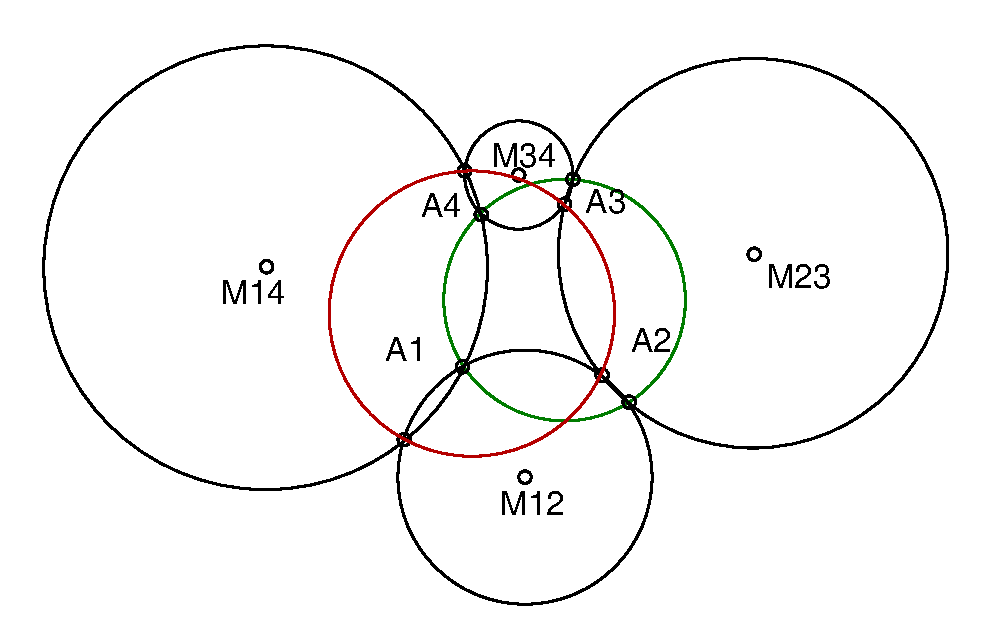
\includegraphics[width=6cm]{linz-02/Miquel.eps}\\
  Figure 3: The Miquel Circle\vskip10pt}\hfill
\parbox[b]{8cm}{
\cite{Li_99a} quotes the problem as hard for the Descartes-Wu approach and
proposes a more geometric solution within the geometric framework developed in
that paper.  The problem has even a constructive solution: Take four points
$A_1,\ldots,A_4$ on a circle around the origin $O$, centers
$M_{12},\ldots,M_{41}$ for circles passing through
$(A_1,A_2),\ldots,(A_4,A_1)$ and compute for each consecutive pair of such
circles the second intersection point (it has rational coordinates in the
parameters $u_1,\ldots,v_4$). } Here is the \GC\ formulation:
\begin{verbatim}
<prooftype> constructive </prooftype>
<parameters> [u1, u2, u3, v1, v2, v3, v4]   </parameters>
<Points>    $O:=Point[0,0]; $A1:=Point[1,0];    </Points>
<coordinates>
$A2:=circle_slider[$O,$A1,u1];
$A3:=circle_slider[$O,$A1,u2];
$A4:=circle_slider[$O,$A1,u3];

$M12:=line_slider[p_bisector[$A1,$A2],v1];
$M23:=line_slider[p_bisector[$A2,$A3],v2];
$M34:=line_slider[p_bisector[$A3,$A4],v3];
$M41:=line_slider[p_bisector[$A4,$A1],v4];

$c12:=pc_circle[$M12,$A1];
$c23:=pc_circle[$M23,$A2];
$c34:=pc_circle[$M34,$A3];
$c41:=pc_circle[$M41,$A4];

$B1:=other_cc_point[$A1,$c12,$c41];
$B2:=other_cc_point[$A2,$c12,$c23];
$B3:=other_cc_point[$A3,$c23,$c34];
$B4:=other_cc_point[$A4,$c34,$c41];
</coordinates>
<conclusion>
$result:=is_concyclic[$B1, $B2, $B3, $B4];
</conclusion>
\end{verbatim}
The simplification of the resulting rational expression in seven parameters
indeed turned out to be very hard and no one of the CAS (Maple, MuPAD, Reduce)
mastered the task.  The situation completely changes if $v_1,\ldots,v_4$ are
assigned random integers (not too big, $<100$). Several runs with differrent
settings always yield 0 (where Maple simplified the new expression much faster
than MuPAD or Reduce).

\section{Implementing the \GC\ Standard} 

For real usability of the {\GC} concept one has to estimate the efforts
required to implement this standard.  Even though there is not yet practical
experience with already existing geometry theorem provers the semantic
similarity of ``foreign'' special geometric proof schemes suggests that such
an interface could easily be implemented.  We suggest to divide that
implementation in two parts as described for the {\GP} packages for different
target CAS: The first part provides (e.g., Perl based) tools to translate GEO
proof schemes into a CAS specific form that fixes requirements of naming and
syntax conventions.  In a second part these translated proof schemes are
passed to a special interface that maps the {\GC} functionality to the target
CAS.

In general, for the second part one has to implement the {\GC} functionality
in the target prover language. This requires extensibility of that language
and access to the source code or interaction with the system developers if
such an interface cannot be added as a supplementary package.

Note that the {\GC} syntax provides not only points but also line and circle
objects as geometric primitives.  It is a special design decision of many
geometry theorem provers, e.g., D.Wang's GEOTHER \cite{Geother}, not to
introduce the latter objects as basic but to take only point objects as
primitives.  A prover extension that respects this spirit can implement lines
and circles as derived objects and represent lines by two base points and
circles by point-center pairs. This is conceptually already present in Wang's
prover and merely should be made explicit. To support such an approach we
removed direct constructors for lines and circles from their homogeneous
coordinates (i.e., the constructors {\tt Line}[$a_1,a_2,a_3$] and {\tt
  Circle}[$a_0,a_1,a_2,a_3$]) from the {\GC} standard in version $1.2$.

A more serious problem arises with geometry theorem provers that do not
support nested function calls. This is typical for systems that contain a
drawing tool, since all intermediate construction steps leave their trace in a
picture. Usually such systems represent and address geometric objects through
explicit identifiers.  To fit generic {\GC} proof schemes with such a prover
nested function calls should be denested. We experimented with a {\GC}
interface to dynamical geometry software (DGS) that uses the Perl 'eval'
mechanism to evaluate nested {\GC} function calls and collects these calls as
a list of construction steps in a generic format. Later on these construction
steps can be mapped to a special DGS, e.g., the system {GEONE$_X$T},
\cite{Geonext}, developed at the University of Bayreuth. 

Experiments with different kinds of tools that support implementations
entailed changes of the {\GC} standard in the past and will entail new
requirements and changes also in the future.  So far the power of the Perl
string manipulation facilities and the {\SD} actions concept were well suited
to support such changes, to scan the GEO records for obsolete proof scheme
commands and to fix them accordingly.

\nocite{Proceedings/ADG-96} \nocite{Proceedings/ADG-98}
\bibliographystyle{plain} %\bibliography{ADG-02,ADG-02.supp}
\begin{thebibliography}{10}

\bibitem{Bachmann_00a}
O.~Bachmann and H.-G. Gr\"{a}be.
\newblock The {\SD} {P}roject: Towards an electronic repository of tools and
  data for benchmarks of computer algebra software.
\newblock Reports on Computer Algebra 27, Jan 2000.
\newblock Centre for Computer Algebra, University of Kaisers\-lautern. See
  \url{http://www.mathematik.uni-kl.de/~zca}.

\bibitem{Books/Chou_88a}
S.-C. Chou.
\newblock {\em Mechanical Geometry Theorem Proving}.
\newblock Reidel, Dortrecht, 1988.

\bibitem{Books/Chou_94a}
S.-C. Chou, X.-S. Gao, and J.-Z. Zhang.
\newblock {\em Machine proofs in geometry}, volume~6 of {\em Series on Applied
  Mathematics}.
\newblock World Scientific Singapore, 1994.

\bibitem{Proceedings/ADG-98}
X.-S. Gao, D.~Wang, and L.~Yang, editors.
\newblock {\em Automated Deduction in Geometry, Beijing 1998}, volume 1669 of
  {\em Lect. Notes Comp. Sci.} Springer, 1999.

\bibitem{gex}
X.-S. Gao et~al.
\newblock {\em Geometry Expert} - a software for dynamic diagram drawing and
  automated geometry theorem proving and discovering, 2002.
\newblock See \url{http://www.mmrc.iss.ac.cn/~xgao/gex.html}.

\bibitem{Geonext}
{GEONE$_X$T} -- a dynamical geometry software, 1998--2002.
\newblock Lehrstuhl f\"ur Mathematik und ihre Didaktik, Univ.~Bayreuth. See
  \url{http://www.geonext.de}.

\bibitem{GeoProver}
H.-G. Gr\"abe.
\newblock {\GP} - a small package for mechanized plane geometry, 1998--2002.
\newblock With versions for Reduce, Maple, MuPAD and Mathematica. Some
  prototypes were compiled in cooperation with M.~Witte. \newblock See
  \url{http://www.informatik.uni-leipzig.de/~compalg/software}.

\bibitem{karlsruhe-02}
H.-G. Gr\"abe.
\newblock The {\SD} benchmark problems collection of polynomial systems.
\newblock In {\em Proceedings of the Workshop on Under- and Overdetermined
  Systems of Algebraic or Differential Equations, Karlsruhe 2002}, pages 57 --
  75, 2002.
\newblock Publ.\ by IAS Karlsruhe. \newblock See also
  \url{http://www.informatik.uni-leipzig.de/~graebe/publications}.

\bibitem{rwca-02}
H.-G. Gr\"abe.
\newblock The {\SD} geometry collection and the {\GP} packages.
\newblock In {\em Proceedings ``8th Rhine Workshop on Computer Algebra''
  (RWCA-02), Mannheim 2002}, pages 173 -- 194, 2002.
\newblock Publ.\ by Univ. Mannheim. \newblock See also
  \url{http://www.informatik.uni-leipzig.de/~graebe/publications}.

\bibitem{IMO}
{The International Mathematical Olympiads}, since 1959.
\newblock See, e.g., \url{http://www.kalva.demon.co.uk/imo.html}.

\bibitem{Kapur_97a}
D.~Kapur.
\newblock Automated geometric reasoning: {Dixon} resultants, {Gr\"obner} bases,
  and characteristic sets.
\newblock In Wang \cite{Proceedings/ADG-96}, pages 1 -- 36.

\bibitem{Li_99a}
C.-Z. Li and J.-Z. Zhang.
\newblock Readable machine solving in geometry and {ICAI} software {MSG}.
\newblock In Gao et~al. \cite{Proceedings/ADG-98}, pages 67 -- 85.

\bibitem{SymbolicData}
{The {\SD} Project}, 2000--2002.
\newblock See \url{http://www.SymbolicData.org} or the mirror at
  \url{http://symbolicdata.uni-leipzig.de}.

\bibitem{Geother}
D.~Wang.
\newblock {\it GEOTHER} - geometry theorem prover, 1990--2001.
\newblock See \url{http://calfor.lip6.fr/~wang/GEOTHER}.

\bibitem{Proceedings/ADG-96}
D.~Wang, editor.
\newblock {\em Automated Deduction in Geometry, Toulouse 1996}, volume 1360 of
  {\em Lect. Notes Comp. Sci.} Springer, 1996.

\bibitem{Wang_96b}
D.~Wang.
\newblock {GEOTHER}: A geometry theorem prover.
\newblock In M.A. McRobbie and J.K. Slaney, editors, {\em Automated deduction
  -- CADE-13}, volume 1104 of {\em LNCS}, pages 166 -- 170, 1996.

\bibitem{Wang_97a}
D.~Wang.
\newblock {Clifford} algebraic calculus for geometric reasoning with
  applications to computer vision.
\newblock In Wang \cite{Proceedings/ADG-96}, pages 115 -- 140.

\bibitem{Books/Wang_01a}
D.~Wang.
\newblock {\em Elimination Methods}.
\newblock Texts and Monographs in Symbolic Computation. Springer, Wien, 2001.

\bibitem{Wu_84b}
W.-T. Wu.
\newblock On the decision problem and the mechanization of theorem-proving in
  elementary geometry.
\newblock In {\em Contemp. Math.}, volume~19, pages 213 -- 234. AMS,
  Providence, Rhode Island, 1984.

\bibitem{Wu_84a}
W.-T. Wu.
\newblock Some recent advances in mechanical theorem proving of geometry.
\newblock In {\em Contemp. Math.}, volume~19, pages 235 -- 241. AMS,
  Providence, Rhode Island, 1984.

\bibitem{Books/Wu_94a}
W.-T. Wu.
\newblock {\em Mechanical Theorem Proving in Geometries}.
\newblock Texts and Monographs in Symbolic Computation. Springer, Wien, 1994.

\bibitem{Wu_99a}
W.-T. Wu.
\newblock Automatic geometry theorem-proving and automatic geometry problem
  solving.
\newblock In Gao et~al. \cite{Proceedings/ADG-98}, pages 1 -- 13.

\bibitem{Books/Wu_01a}
W.-T. Wu.
\newblock {\em Mathematics Mechanization}, volume~489 of {\em Mathematics and
  its Applications}.
\newblock Science Press, Beijing, and Kluwer Acad. Publ., Dordrecht, 2000.

\end{thebibliography}


\end{document}

